\subsection{Settimo sprint}

\begin{minipage}{\textwidth}
  Di seguito è riportata la distribuzione delle ore per ciascun membro del team, accumulate in totali per persona e per ruolo:
  \begin{table}[H]
    \begin{tabularx}{\textwidth}{|c|*{6}{>{\centering}X|}c|}
      \hline
      \multicolumn{8}{|c|}{\textbf{Consuntivo orario}} \\
      \hline
      \textbf{Membro del team} & \textbf{Re} & \textbf{Am} & \textbf{An} & \textbf{Pt} & \textbf{Pr} & \textbf{Ve} & \textbf{Totale per persona} \\
      \hline
      Riccardo Cavalli & 0 & 0 & 0 & 0 & 3 & 2 & 5 \\
      \hline
      Raul Pianon & 0 & 2 & 0 & 0 & 1 & 1 & 4 \\
      \hline
      Martina Dall'Amico & 0 & 0 & 0 & 0 & 3 & 0 & 3 \\
      \hline
      Marco Cristo & 0 & 1 & 0 & 0 & 0 & 2 & 3 \\
      \hline
      Sebastiano Lewental & 1 & 0 & 0 & 0 & 2 & 1 & 4 \\
      \hline
      Mattia Zecchinato & 2 & 3 & 0 & 0 & 0 & 0 & 5 \\
      \hline
      Tommaso Stocco & 0 & 4 & 0 & 0 & 0 & 0 & 4 \\
      \hline
      \textbf{Totale ore per ruolo} & 3 & 10 & 0 & 0 & 9 & 6 & \textbf{28} \\
      \hline
    \end{tabularx}
    \caption{Sprint 7 - Consuntivo orario}
  \end{table}
  \end{minipage}

  \begin{figure}[H]
    \centering
    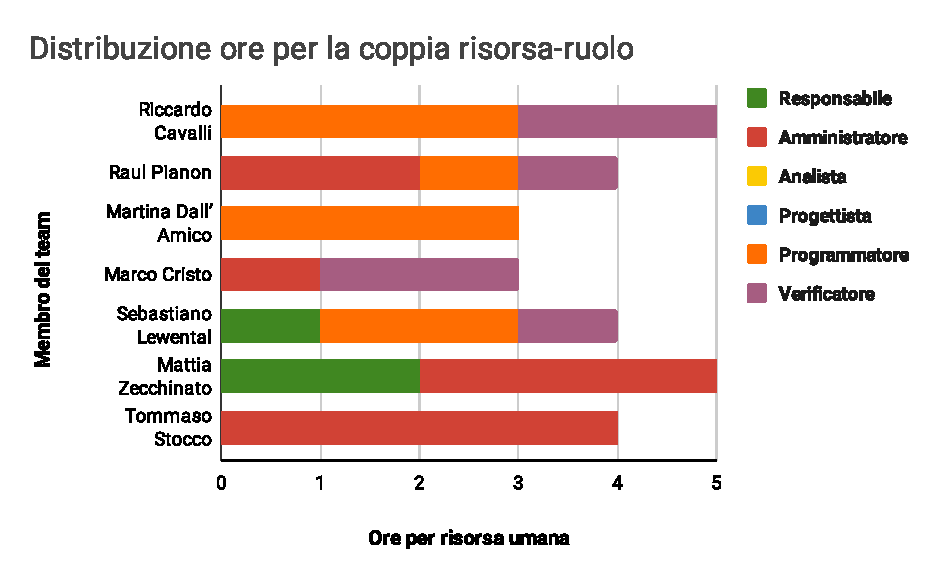
\includegraphics[width=0.90\textwidth]{assets/Consuntivo/Sprint-7/distribuzione_ore_risorsa_ruolo.pdf}
    \caption{Sprint 7 - Istogramma della distribuzione oraria per la coppia risorsa-ruolo}
  \end{figure}

  \begin{figure}[H]
    \centering
    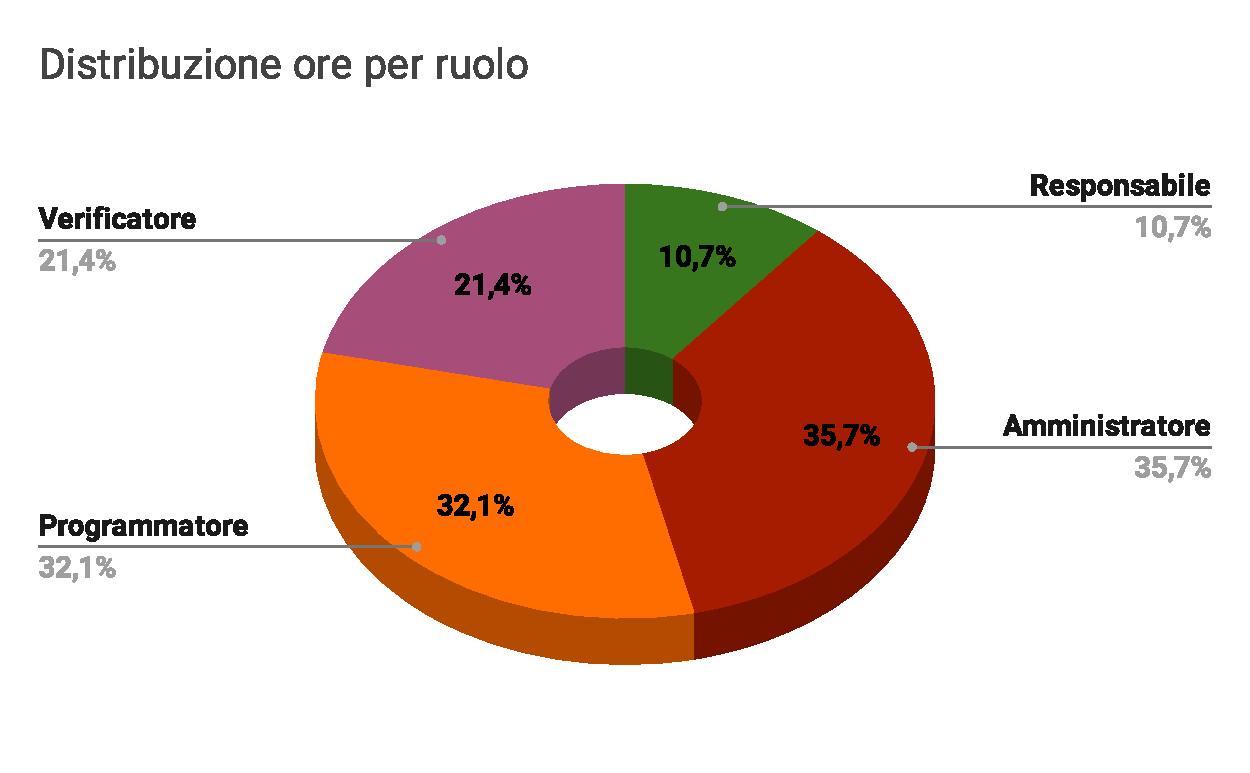
\includegraphics[width=0.90\textwidth]{assets/Consuntivo/Sprint-7/distribuzione_ore_ruolo.pdf}
    \caption{Sprint 7 - Areogramma della distribuzione oraria per ruolo}
  \end{figure}

  \begin{minipage}{\textwidth}
  Di seguito è riportato il consuntivo economico del settimo \glossario{sprint}:
  \begin{table}[H]
  \begin{adjustwidth}{-0.5cm}{-0.5cm}
    \centering
    \begin{tabular}{|P{2.9cm}|P{2.3cm}|P{2.5cm}|P{2.3cm}|>{\arraybackslash}P{2.5cm}|}
      \hline
      \multicolumn{5}{|c|}{\textbf{Consuntivo economico}} \\
      \hline
      \textbf{Ruolo} & \textbf{Ore per ruolo} & \textbf{Delta ore preventivo - consuntivo} & \textbf{Costo (in \texteuro)} & \textbf{Delta costo preventivo - consuntivo (in \texteuro)} \\
      \hline
      \Responsabile[U]{} & 3 & 1 & 90,00 & 30,00 \\ \hline
      \Amministratore[U]{} & 10 & -2 & 200,00 & -40,00 \\ \hline
      \Analista[U]{} & 0 & 1 & 0,00 & 25,00 \\ \hline
      \Progettista[U]{} & 0 & 0 & 0,00 & 0,00 \\ \hline
      \Programmatore[U]{} & 9 & -2 & 135,00 & -30,00 \\ \hline
      \Verificatore[U]{} & 6 & 2 & 90,00 & 30,00 \\ \hline
      \textbf{Totale} & \textbf{28} & 0 & \textbf{515,00} & 15,00 \\ \hline
      \textbf{Restante} & 338 & / & 6.775,00 & / \\ \hline
      \textbf{Sprint pregressi} & 280 & / & 5.730,00 & / \\ \hline
    \end{tabular}
    \caption{Sprint 7 - Consuntivo economico}
  \end{adjustwidth}
  \end{table}
  \end{minipage}

  \begin{figure}[H]
    \centering
    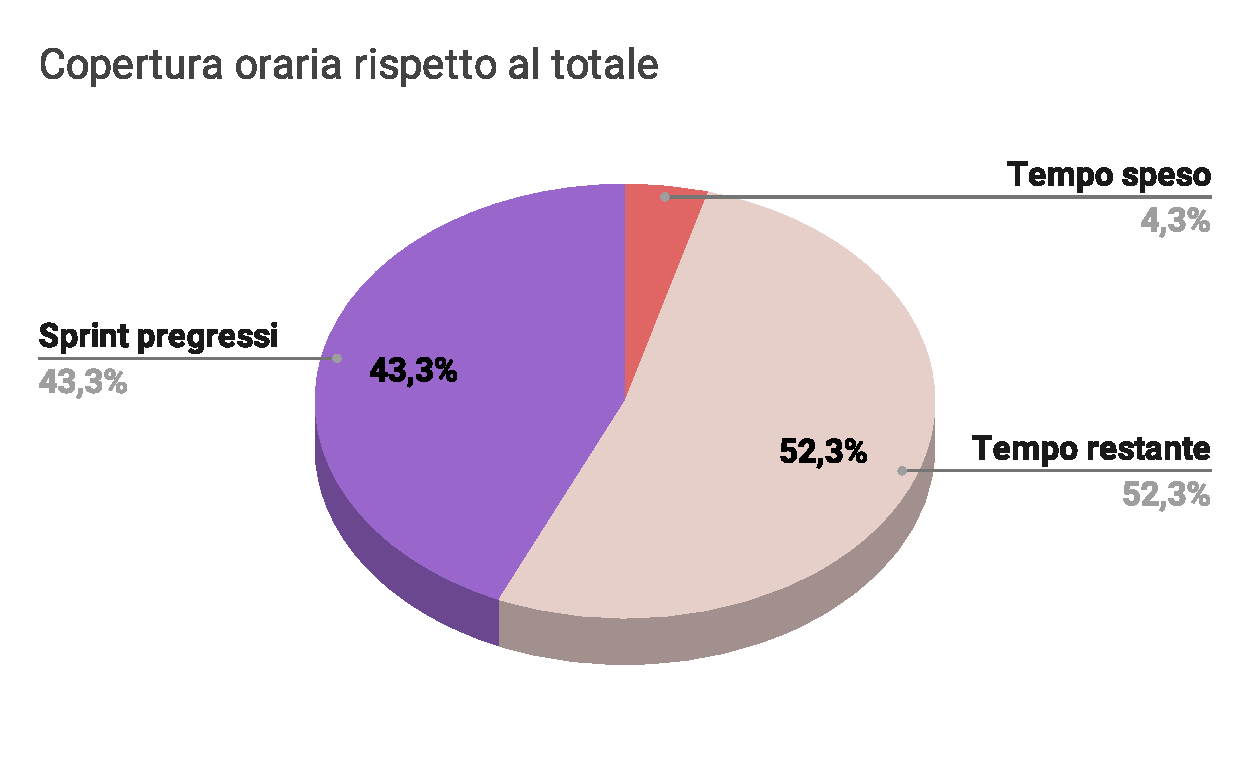
\includegraphics[width=0.90\textwidth]{assets/Consuntivo/Sprint-7/copertura_oraria.pdf}
    \caption{Sprint 7 - Areogramma del tempo speso (in ore) rispetto al totale}
  \end{figure}

  \begin{figure}[H]
    \centering
    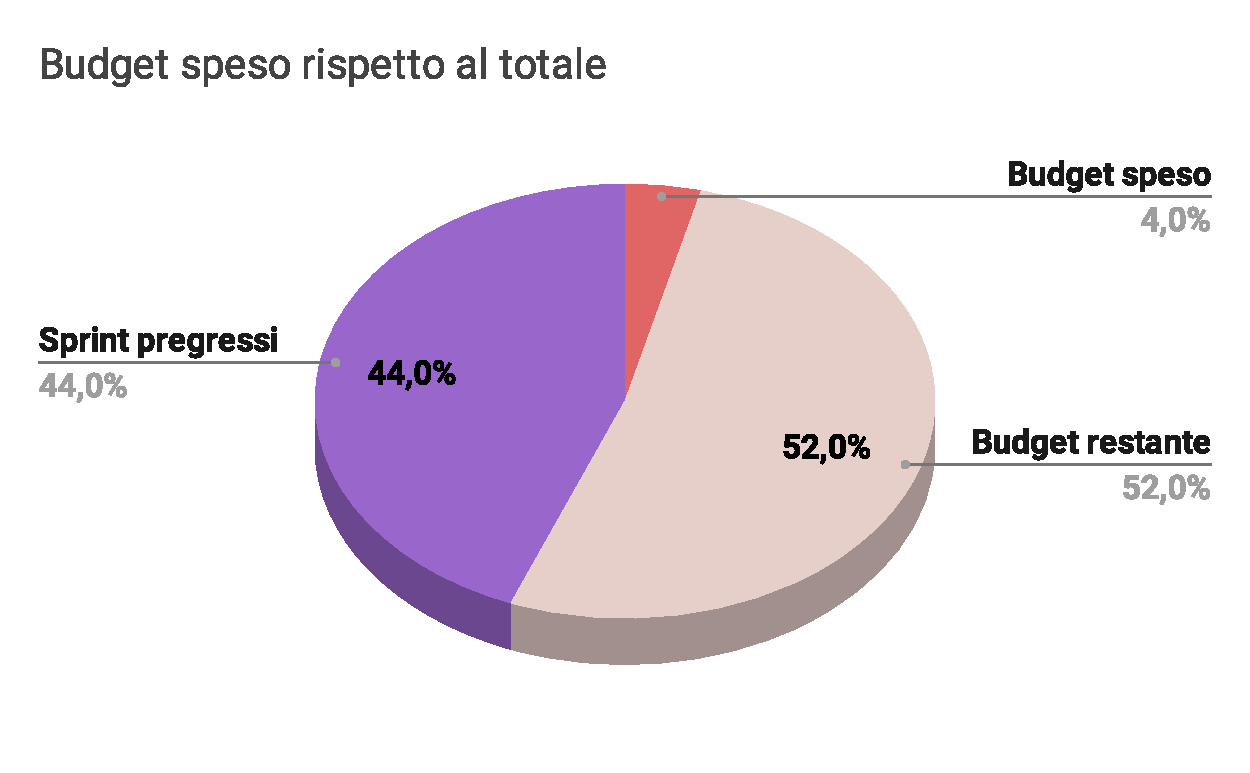
\includegraphics[width=0.90\textwidth]{assets/Consuntivo/Sprint-7/budget_speso.pdf}
    \caption{Sprint 7 - Areogramma del budget speso rispetto al totale}
  \end{figure}

  \begin{minipage}{\textwidth}
    Di seguito sono riportate le ore rimanenti per la coppia risorsa-ruolo:
    \begin{table}[H]
      \begin{tabularx}{\textwidth}{|c|*{6}{>{\centering}X|}c|}
        \hline
        \multicolumn{8}{|c|}{\textbf{Ore rimanenti per la coppia risorsa-ruolo}} \\
        \hline
        \textbf{Membro del team} & \textbf{Re} & \textbf{Am} & \textbf{An} & \textbf{Pt} & \textbf{Pr} & \textbf{Ve} & \textbf{Totale per persona} \\
        \hline
        Riccardo Cavalli & 0 & 0 & 3 & 14 & 13 & 13 & 43 \\
        \hline
        Raul Pianon & 2 & 5 & 1 & 20 & 9 & 9 & 46 \\
        \hline
        Martina Dall'Amico & 5 & 2 & 1 & 14 & 16 & 12 & 50 \\
        \hline
        Marco Cristo & 2 & 8 & 0 & 17 & 10 & 11 & 48 \\
        \hline
        Sebastiano Lewental & 5 & 4 & 2 & 11 & 12 & 15 & 49 \\
        \hline
        Mattia Zecchinato & 7 & 3 & 3 & 11 & 12 & 13 & 49 \\
        \hline
        Tommaso Stocco & 5 & 0 & 3 & 20 & 9 & 14 & 51 \\
        \hline
        \textbf{Totale ore per ruolo} & 26 & 23 & 13 & 107 & 82 & 87 & \textbf{338} \\
        \hline
      \end{tabularx}
      \caption{Sprint 7 - Ore rimanenti per la coppia risorsa-ruolo}
    \end{table}
  \end{minipage}

\subsubsection{Revisione delle attività}

\par Nell'arco del settimo \glossario{sprint}, il team ha svolto le seguenti attività:
\begin{itemize}
  \item Revisione consuntivi \PdP;
  \item Aggiunta metriche alle \NdP;
  \item Completamento sezioni incomplete \NdP;
  \item Stesura sezione test nel \PdQ;
  \item Stesura dei verbali interni;
  \item Gestione stato Utente/Tecnico a \glossario{front-end};
  \item Creazione interfaccia Chat a \glossario{front-end};
  \item Implementazione funzioni per generare il \glossario{prompt} e mostrarlo a \glossario{front-end}.
\end{itemize}

\subsubsection{Retrospettiva}

\par Di seguito sono riportati i risultati del questionario di valutazione dello \glossario{sprint}:
\begin{itemize}
  \item Organizzazione dello \glossario{sprint}\ - Valutazione: 8;
  \item Conduzione dei meeting interni - Valutazione: 8;
  \item Conduzione dei meeting esterni - Valutazione: 8;
  \item Impegno e partecipazione dei singoli membri - Valutazione: 3;
  \item La quasi totalità dei membri del team era a conoscenza delle proprie mansioni;
  \item La numerosità delle riunioni è risultata adeguata per tutti i membri del gruppo;
  \item Le riunioni sono state organizzate quasi sempre con il giusto preavviso;
  \item Il rapporto ore spese/ore produttive si sta notevolmente equilibrando;
  \item La produttività è stata ragioneole considerando le criticità della sessione;
  \item È diffusa l'idea di programmare incontri in presenza più frequenti.
\end{itemize}

\vspace{0.5\baselineskip}
\par A seguire le \textbf{analisi a posteriori} del settimo \glossario{sprint}:
\begin{itemize}
  \item La sessione di esami ha impattato sulla quantità di lavoro svolto, come previsto;
  \item Durante la sessione è risultato più complicato organizzare incontri ripetuti con una partecipazione completa del gruppo, per cui si è preferito organizzare un incontro ad inizio \glossario{sprint} di allineamento e poi lasciare l'organizzazione per singoli ruoli;
  \item A causa degli impegni è stato più complicato gestire le risorse disponibili e l'aggiornamento quotidiano, per questo motivo il \Responsabile{} ha impostato dei reminder automatici per ricordare al gruppo la compilazione delle attività e progressi svolti;
  \item La modifica di durata degli sprint a circa 1 settimana è risultata essere abbastanza complessa nella gestione di attività individuali, soprattutto durante la sessione di esami. Per questo motivo si è deciso di procedere a seguito della \glossario{RTB} con la ripianificazione di sprint di lunghezza di 2 settimane, in modo da permettere una più semplice organizzazione degli impegni, non inficiando però l'organizzazione del lavoro collaborativo.
\end{itemize}

\subsubsection{Aggiornamento pianificazione e preventivo}
\par Il team ha definito un piano d'azione per migliorare l'organizzazione e la produttività del prossimo \glossario{sprint}:
\begin{itemize}
  \item Proseguire con la programmazione di un incontro in presenza ogni due settimane.
\end{itemize}

\paragraph*{Pianificazione futura:}
\par A causa degli impegni universitari, il gruppo ha deciso di non aumentare il carico di lavoro individuale, ma di incrementare in modo significativo la produttività dopo la conclusione della RTB.

\paragraph*{Preventivo "a finire" (\sezione{sec:stima_temporale}):}
\par Il team ha confermato la scelta di svolgere la revisione \glossario{RTB} dopo la sessione di esami; una volta terminata la RTB, il gruppo valuterà se ridistribuire le ore per ruolo.

\paragraph*{Gestione dei rischi (\sezione{sec:analisi_rischi}):}
\par Nel corso del settimo \glossario{sprint}, alcune contromisure si sono rivelate insufficienti a mitigare i rischi emersi:
\begin{itemize}
  \item \textbf{RT4 - Connettività limitata}: l'impossibilità di alcuni membri del gruppo a partecipare alle riunioni ha complicato la comunicazione interna e la gestione del progetto. Per mitigare tale rischio, il team ha deciso di incrementare la frequenza degli incontri in presenza.
\end{itemize}

\vspace{0.5\baselineskip}
\par Di seguito sono elencati i rischi gestiti con successo:
\begin{itemize}
  \item \textbf{RT3 - Malfunzionamenti software}: durante l'esecuzione dei test per il \glossario{Proof of Concept}, alcuni componenti del gruppo hanno riscontrato problemi tecnici legati all'utilizzo delle tecnologie e librerie. Il rischio è stato mitigato mediante l'organizzazione di riunioni in presenza che hanno favorito una comunicazione diretta e interventi più mirati;
  \item \textbf{RO2 - Collaborazione}: sostenere una collaborazione continua durante la sessione di esami è risultato difficile a causa della limitata disponibilità dei membri del team; è stato necessario organizzare riunioni più concise e definire task mirati. Tuttavia, questa pianificazione si è rivelata adeguata, grazie soprattutto all'esperienza maturata nel corso degli \glossario{sprint} precedenti, alleviando il carico individuale senza compromettere l'avanzamento del progetto;
  \item \textbf{RO1 - Periodi di rallentamento}: il team ha avuto difficoltà a conciliare l'avanzamento del progetto e lo studio personale; pertanto, le ore produttive individuali sono state ridotte. Trattandosi di un rischio preventivato, il gruppo è riuscito a mantenere un flusso di lavoro regolare;
  \item \textbf{RO6 - Risorse disponibili ma non impiegate}: nonostante il team abbia perso alcune ore potenzialmente produttive, gli incontri in presenza hanno compensato tali perdite.
\end{itemize}

